\chapter{Tools for Query Building}
\label{chap:tools_query_building}

Discovering digital art collections encompasses a wide array of possibilities, each with its unique interpretations and implementations. This research, however, primarily centers on the facilitation aspect of this discovery process. The CoGhent collections undoubtedly harbor a treasure trove of potentially captivating insights, yet professionals and art enthusiasts can only unlock these treasures if they can formulate the right SPARQL queries. This task is far from simple, particularly when considering that these individuals might lack the technical proficiency required to construct such queries. Consequently, this chapter introduces and partially develops two conceptual web applications designed to significantly alleviate the technical complexities of query formulation for users.

The first application draws inspiration from the existing CoGhent Query Builder proposed in Section~\ref{subsec:coghent_query_builder}. The fundamental concept remains unchanged: users are presented with a list of properties, and based on their selections, the application constructs a query with the necessary triple patterns to retrieve the desired data. However, the \textit{enhanced} iteration of this application takes two further strides. Firstly, it introduces modularity by ensuring that the properties and their corresponding triple patterns are not hard-coded into the application. Instead, they are provided as sequences of predicates through JSON files. Secondly, the application supports the generation of \textit{cross-dataset queries} that can be effectively resolved through a link traversal engine, as elaborated in Chapter~\ref{chap:coghent_link_traversal}.

The second application targets users with a slightly more advanced understanding of RDF. It empowers them to explore the predicate sequences of properties of interest themselves. This exploration journey begins with an RDF resource provided by the user. From this initial \textit{root} resource, users can progressively construct a tree comprising of predicates and objects. Based on users' choices, the application executes queries to fetch the predicates and objects associated with an already-present resource in the tree. As users gain a deeper understanding of the data accessible through the given root resource, they can select specific objects within the tree. The application then deduces the predicate sequences leading from the root resource to these chosen objects and subsequently generates a corresponding query. Crucially, since this query solely relies on predicate sequences, it empowers users to perform a generalized inquiry on their entire dataset(s), not just the resource specified at the beginning of the process.

Both of these applications are briefly introduced in Sections~\ref{sec:new_query_builder} and~\ref{sec:discovering_predicate_sequences}, respectively, by discussing their main features and most essential implementation details. For the complete implementations, readers are referred to their respective GitHub repositories: \url{https://github.com/thesis-Martijn-Bogaert-2022-2023/sparql-query-builder-ui} and \url{https://github.com/thesis-Martijn-Bogaert-2022-2023/rdf-predicates-explorer}. However, prior to this, Section~\ref{sec:building_queries_predicate_sequences} first covers the fundamental functionality shared by both web applications. As to avoid repeating code and to ensure separation of concerns, this functionality lives on its own and is incorporated into the other two applications by importing its implementation as a package. The detailed implementation of this essential tool can be found in the following GitHub repository: \url{https://github.com/thesis-Martijn-Bogaert-2022-2023/sparql-query-builder}.

\section{Building Queries from Predicate Sequences}
\label{sec:building_queries_predicate_sequences}

To provide user-oriented applications with the capability to obtain the corresponding query based on an input of predicate sequences, this section introduces a Node.js application that accomplishes precisely that. The application does not have a user interface; it solely exports a function that performs the described functionality. This allows other Node.js applications to use the function by installing the application as a package.

The actual implementation can be found in the following GitHub repository:
\begin{center}
    \url{https://github.com/thesis-Martijn-Bogaert-2022-2023/sparql-query-builder}.
\end{center}

\subsection{Arrays of Triple Patterns}

The simplest but somewhat naive way to build queries in the application is by maintaining the necessary triple patterns for each \textit{property} they represent in a single string. Based on the properties selected by the user, the application can then place the corresponding strings one by one in the \mintinline{text}{WHERE} clause of a new query. However, starting from such completely hard-coded \textit{chunks} of triple patterns not at all meets the requirement of working with \textit{predicate sequences}, makes it difficult to \textit{clean up} the query, and is simply no elegant solution.

The next logical approach is to keep an array of strings for each property, with each string representing a single triple pattern. Code Fragment~\ref{lst:where_statements_array} provides an example of what such an array might look like. Note that the array itself effectively becomes the value of a key-value pair, the key being the property name. This allows to \textit{feed} the function responsible for the actual query building with a dictionary of such key-value pairs.

\begin{listing}[htbp]
    \begin{minted}[samepage,fontsize=\small]{js}
objectname: [
    '?s cidoc:P41i_was_classified_by ?classified.',
    '?classified cidoc:P42_assigned ?assigned.',
    '?assigned skos:prefLabel ?objectname.',
]
    \end{minted}
    \caption{WHERE clause statements to query for \textit{objectname} stored as elements in an array}
    \label{lst:where_statements_array}
\end{listing}

An important and convenient feature of SPARQL is the ability to use prefixes. Code Fragment~\ref{lst:where_statements_array}, for instance, assumes that the provided triple patterns are already utilizing prefixes. Naturally, in this case, the application should construct a query that begins with the necessary \mintinline{text}{prefix} statements. The simplest, yet again naive, way to achieve this is by including the same set of \mintinline{text}{prefix} statements at the start of each query. Code Fragment~\ref{lst:prefix_statements_original} illustrates what this set of \mintinline{text}{prefix} statements might look like.

\begin{listing}[htbp]
    \begin{minted}[samepage,fontsize=\small]{sparql}
PREFIX cidoc:<http://www.cidoc-crm.org/cidoc-crm/>
PREFIX adms:<http://www.w3.org/ns/adms#>
PREFIX skos:<http://www.w3.org/2004/02/skos/core#>
PREFIX la:<https://linked.art/ns/terms/>
    \end{minted}
    \caption{All possible PREFIX statements of the original CoGhent Query Builder}
    \label{lst:prefix_statements_original}
\end{listing}

It hardly needs mentioning that the solutions described above come with several issues. First, breaking down the \textit{chunks} of triple patterns into separate array members still does not allow for a clean query generation process. Second, hard-coded prefixes hinder the modularity of the app. After all, only accepting triple statements with prefixes from such a limited predefined list is hardly user-friendly. Moreover, even if the app aims to accommodate as many types of prefixes as possible, the question arises: how extensive should that list - and thus each query - become?

\subsection{Arrays of Predicates}

To address both of these shortcomings, an improved approach is proposed. It is important to realize that due to the nature of the queries being formulated in this research, only the predicate of each triple pattern is of real importance. The subjects and objects are consistently variables, and storing their names along with the predicate does not serve much purpose. Therefore, the elements in each property's array do not need to correspond directly to explicit triple patterns, but solely to predicates. This really brings the concept of \textit{predicate sequences} to the forefront. Additionally, to have a better understanding of which prefixes are potentially used, these can also be extracted from the predicate strings and stored separately. With these observations in mind, Code Fragment~\ref{lst:where_statements_array_predicates} introduces a new data structure. In it, each property to be included in the query, holds an array of objects. In turn, each of these objects includes a mandatory predicate field and, in case the latter is no URI, a prefix field as well.

\begin{listing}[htbp]
    \begin{minted}[samepage,fontsize=\small]{js}
objectname: [
    { prefix: 'cidoc', predicate: 'P41i_was_classified_by' },
    { prefix: 'cidoc', predicate: 'P42_assigned' },
    { prefix: 'skos', predicate: 'prefLabel' },
]
    \end{minted}
    \caption{Prefixes and predicates for WHERE clause statements to query for \textit{objectname} stored as elements in an array}
    \label{lst:where_statements_array_predicates}
\end{listing}

Immediately, it becomes apparent that using this new data structure is much more elegant than the initially proposed approach. However, the downside is that the query building function now has more work to do. Since variable names are no longer specified, the function needs to generate them. This can be approached in two ways.

Firstly, the function could use a generic variable name like \mintinline{text}{var} and append an ever increasing number to it. The major drawback of this solution, though, is that generic variable names can make the query less readable. For instance, while Code Fragment~\ref{lst:where_statements_objects_numbers} required introducing \textit{only} four such variable names, it becomes evident that a larger number of them would make the final query less user-friendly.

\begin{listing}[htbp]
    \begin{minted}[samepage,fontsize=\small]{sparql}
# Objectname
?var1 cidoc:P41i_was_classified_by ?var2.
?var2 cidoc:P42_assigned ?var3.
?var3 skos:prefLabel ?var4.
    \end{minted}
    \caption{WHERE clause statements with object variable names constructed using numbers}
    \label{lst:where_statements_objects_numbers}
\end{listing}

As a second approach, the function could use variable names determined by the preceding variable names and predicates. Code Fragment~\ref{lst:where_statements_objects_long} demonstrates that this type of variable naming indeed clearly indicates their purpose. However, in terms of user-friendliness, this approach scores even worse than the previous one. Queries quickly become overloaded with overly long variable names, rendering them barely understandable and certainly not readable.

\begin{listing}[htbp]
    \begin{minted}[samepage,fontsize=\small]{sparql}
# Objectname
?s
    cidoc:P41i_was_classified_by
        ?s_cidoc_P41i_was_classified_by.
?s_cidoc_P41i_was_classified_by
    cidoc:P42_assigned
        ?s_cidoc_P41i_was_classified_by_cidoc_P42_assigned.
?s_cidoc_P41i_was_classified_by_cidoc_P42_assigned
    skos:prefLabel
        ?s_cidoc_P41i_was_classified_by_cidoc_P42_assigned_skos_prefLabel.
    \end{minted}
    \caption{WHERE clause statements with object variable names constructed from preceding statements}
    \label{lst:where_statements_objects_long}
\end{listing}

It is evident that none of the approaches mentioned above is the optimal solution. Therefore, in Section~\ref{subsec:variable_names_property_path_sequences}, things are being approached differently one last time. However, before proceeding, another dilemma needs to be addressed. Namely, when multiple properties are involved in a query, it is entirely possible that parts of their \textit{paths} toward their respective end objects, overlap. In other words, it is plausible that the query function needs to add the same triple pattern to the \mintinline{text}{WHERE} clause multiple times. Code Fragment~\ref{lst:where_statements_overlapping} illustrates what such a query might look like. Indeed, in principle, the second occurrence of the triple pattern \mintinline{text}{?o cidoc:P108i_was_produced_by ?produced} is redundant. After all, once a SPARQL engine reaches this triple pattern, it will utilize the existing bindings for the variables \mintinline{text}{?o} and \mintinline{text}{?produces}, rendering this triple pattern dispensable.

\begin{listing}[htbp]
    \begin{minted}[samepage,fontsize=\small]{sparql}
# Place
?o cidoc:P108i_was_produced_by ?produced.
?produced cidoc:P7_took_place_at ?tookplace.
?tookplace la:equivalent ?plaatsequivalent.
?plaatsequivalent skos:prefLabel ?plaats.
# Date
?o cidoc:P108i_was_produced_by ?produced.
?produced cidoc:P4_has_time-span ?timespan.
    \end{minted}
    \caption{WHERE clause statements with overlapping statements}
    \label{lst:where_statements_overlapping}
\end{listing}

Code Fragment~\ref{lst:where_statements_no_overlapping} depicts the same query as displayed in Code Fragment~\ref{lst:where_statements_overlapping}, but without duplicate triple patterns. Such a query is indeed more compact, but the query-building process becomes slightly more complicated. For instance, to keep track of the various predicates already used, along with their subject and object variables, the entered \textit{flat} predicates dictionary could be transformed into a tree structure, where branches represent unique predicates and nodes denote intermediary variable names. This approach would subsequently allow for building queries void of duplicate triple patterns. However, one might question whether it is worthwhile to implement such \textit{complex} logic. In fact, even though permitting duplicate triple patterns might potentially lengthen the resulting queries, it simultaneously contributes to more comprehensible and lucid queries. This is evidenced by the query in Code Fragment~\ref{lst:where_statements_overlapping}: it is readily apparent, both for the \textit{place} property and the \textit{data} property, which \textit{paths} must be traversed to retrieve their respective objects of interest. Bearing this in mind, this research prioritizes the creation of these \textit{clear} queries.

\begin{listing}[htbp]
    \begin{minted}[samepage,fontsize=\small]{sparql}
# Place
?o cidoc:P108i_was_produced_by ?produced.
?produced cidoc:P7_took_place_at ?tookplace.
?tookplace la:equivalent ?plaatsequivalent.
?plaatsequivalent skos:prefLabel ?plaats.
# Date
?produced cidoc:P4_has_time-span ?timespan.
    \end{minted}
    \caption{WHERE clause statements without overlapping statements}
    \label{lst:where_statements_no_overlapping}
\end{listing}

\subsection{User-Defined Variable Names and Property Path Sequences}
\label{subsec:variable_names_property_path_sequences}

As discussed in the previous section, a way must be devised to handle the usage of variable names. Since this research aims to assist individuals without the necessary technical knowledge in comprehending too complex queries, two additional functionalities are introduced. These functionalities aim to both condense queries and make them more intelligible.

To fulfill the first objective, property path sequences are employed. These sequences essentially concatenate consecutive predicates, eliminating the need for variable names. To achieve the second objective, users are provided with the option to add an \mintinline{text}{object_variable_name} key to the triple pattern descriptions in the properties dictionary. For instance, when the query-building function encounters an \mintinline{text}{object_variable_name}, it will not concatenate the next predicate to the current one using a property path sequence. Instead, it will use the specified variable name for the object of the current triple pattern, as well as for the subject of the next one. Additionally, a \mintinline{text}{subject_variable_name} can also be included. However, to avoid clashes with potential \mintinline{text}{object_variable_name}s, this will only be respected for the first triple pattern description in an array. This should provide the capability to deviate the starting point of a sequence of triple patterns from the \textit{default} starting point.

In principle, the functionality described above should suffice for building clear, albeit very simple queries. For that reason, before discussing a handful additional features in Sections~\ref{subsec:filter_optional_properties} and~\ref{subsec:limit_offset} Code Fragments~\ref{lst:properties_prefixes_query_build_function} and~\ref{lst:query_generated_edge_cases} are introduced. Code Fragment~\ref{lst:properties_prefixes_query_build_function} presents two dictionaries intended to be passed to the query-building function. The \mintinline{text}{properties} dictionary attempts to illustrate the concepts discussed earlier. Specifically, the dictionary outlines \textit{paths} to several objects of interest. For the \mintinline{text}{title} and \mintinline{text}{description} properties, only one predicate is needed each, while the \mintinline{text}{objectname} and \mintinline{text}{association} properties require three and four predicates, respectively. For each element in the property arrays, a \mintinline{text}{predicate} is provided; logically, this is the only mandatory named value. Additionally, prefixes are added where necessary. The query-building function will place these prefixes before their corresponding predicates. To ensure a functional query, however, it is assumed that the URIs representing the prefixes are provided separately to the query-building function. The latter will subsequently use them to create \mintinline{text}{PREFIX} statements at the beginning of the query. Moving on, no beginning array element is assigned a \mintinline{text}{subject_variable_name}, which should result in a query where each \textit{path} starts from the same subject variable. However, two \mintinline{text}{object_variable_name} specifications are provided. Their corresponding variable names should appear in the resulting query, essentially \textit{breaking} the regular property path sequences. Indeed, as depicted in Code Fragment~\ref{lst:query_generated_edge_cases}, the output of the query-building function matches the expectations perfectly.

\begin{listing}[htbp]
    \begin{minted}[samepage,fontsize=\small]{js}
const properties = {
    title: [
        { prefix: 'cidoc', predicate: 'P102_has_title' }
    ],
    description: [
        { prefix: 'cidoc', predicate: 'P3_has_note', object_variable_name: 'note' },
    ],
    objectname: [
        { prefix: 'cidoc', predicate: 'P41i_was_classified_by' },
        { prefix: 'cidoc', predicate: 'P42_assigned' },
        { predicate: 'http://www.w3.org/2004/02/skos/core#prefLabel' },
    ],
    association: [
        { prefix: 'cidoc', predicate: 'P128_carries' },
        { prefix: 'cidoc', predicate: 'P129_is_about', object_variable_name: 'about' },
        { prefix: 'cidoc', predicate: 'P2_has_type' },
        { predicate: 'http://www.w3.org/2004/02/skos/core#prefLabel' },
    ],
};

const prefixes = {
    cidoc: 'http://www.cidoc-crm.org/cidoc-crm/',
};
    \end{minted}
    \caption{Properties and prefixes ready to be consumed by query building function}
    \label{lst:properties_prefixes_query_build_function}
\end{listing}

\begin{listing}[htbp]
    \begin{minted}[samepage,fontsize=\small]{sparql}
PREFIX cidoc:<http://www.cidoc-crm.org/cidoc-crm/>
PREFIX skos:<http://www.w3.org/2004/02/skos/core#>

SELECT ?title ?note ?objectname ?association

WHERE {
    # title
    ?human_made_object cidoc:P102_has_title ?title.
    
    # description
    ?human_made_object cidoc:P3_has_note ?note.
    
    # objectname
    ?human_made_object
        cidoc:P41i_was_classified_by/cidoc:P42_assigned/skos:prefLabel
            ?objectname.
            
    # association
    ?human_made_object cidoc:P128_carries/cidoc:P129_is_about ?about.
    ?about cidoc:P2_has_type/skos:prefLabel ?association.
}
    \end{minted}
    \caption{SPARQL query generated from input displayed in Code Fragment \ref{lst:properties_prefixes_query_build_function}}
    \label{lst:query_generated_edge_cases}
\end{listing}

\subsection{Filtered and Optional Properties}
\label{subsec:filter_optional_properties}

As with the original CoGhent Query Builder, this application should provide the ability to filter and/or make properties optional. While, technically, a SPARQL query can have these specifications defined anywhere in its WHERE clause, in the orginal CoGhent Query Builder's and this application's case, these specifications are intended to be defined per \textit{property}. This only makes sense, as from the perspective of simplicity and consistency, both applications aim to abstract the complexities of query building to a large extent. Therefore, it might be inappropriate to provide users with the ability to manipulate the abstracted triple patterns at the beginning. Besides, once the query is generated, users can obviously still modify it as they wish.

To include the filtering functionality, one approach is to provide a new dictionary to the query-building function where property names can be listed along with their filter details. However, introducing a third dictionary might become a bit cluttered for developers. Therefore, an alternative approach is to incorporate the filter details into the existing \mintinline{text}{properties} array. For this, a slight modification to the data structure is needed. Code Fragment~\ref{lst:properties_filter_optionals} demonstrates what this entails. Specifically, the array containing predicate information is no longer the direct value of its predicate key. Instead, the value of the predicate key becomes a dictionary that has room for a \mintinline{text}{statements} key, which in turn houses the original array of statements.

\begin{listing}[htbp]
    \begin{minted}[samepage,fontsize=\small]{js}
const properties = {
    title: {
        statements: [
            { prefix: 'cidoc', predicate: 'P102_has_title' }
        ],
    },
    description: {
        statements: [
            { prefix: 'cidoc', predicate: 'P3_has_note', object_variable_name: 'note' },
        ],
        filters: { string: 'luchter', language: 'nl' },
        optional: true,
    },
};
    \end{minted}
    \caption{Example of properties dictionary to illustrate use of filters and optionals}
    \label{lst:properties_filter_optionals}
\end{listing}

Now that each property in the properties array can host various types of data, there is finally space for a \mintinline{text}{filters} key. This key specifies a new dictionary where multiple types of filters can be accommodated. In fact, unlike the original CoGhent Query Builder, this opens up the possibility of allowing different kinds of filters alongside a regex-based and case-insensitive \mintinline{text}{string} filter. Of course, this is provided that the query-building function knows how to handle them. At the time of publishing this research, an additional feature has been implemented which allows specifying a \mintinline{text}{language} filter value. Code Fragment~\ref{lst:query_generated_filters_optionals} presents the corresponding query based on the properties dictionary in Code Fragment~\ref{lst:properties_filter_optionals} and demonstrates how the language filter is reflected in the query.

\begin{listing}[htbp]
    \begin{minted}[samepage,fontsize=\small]{sparql}
PREFIX cidoc:<http://www.cidoc-crm.org/cidoc-crm/>

SELECT ?title ?note

WHERE {
    # title
    ?human_made_object cidoc:P102_has_title ?title.
    
    # description
    OPTIONAL {
        ?human_made_object cidoc:P3_has_note ?note.
        
        FILTER(REGEX(?note, "luchter", "i"))
        FILTER(LANG(?note) = "nl")
    }
}
    \end{minted}
    \caption{SPARQL query generated from input displayed in Code Fragment \ref{lst:properties_filter_optionals}}
    \label{lst:query_generated_filters_optionals}
\end{listing}

Code Fragments~\ref{lst:properties_filter_optionals} and~\ref{lst:query_generated_filters_optionals} also illustrate how a property can be made optional. This can be achieved simply by adding the \mintinline{text}{optional} key to the property details and setting its value to \mintinline{text}{true}.

\subsection{Limit and Offset}
\label{subsec:limit_offset}

Finally, the application is also capable of adding a \mintinline{text}{LIMIT} and/or \mintinline{text}{OFFSET} statement to the query. Their corresponding parameters, \mintinline{text}{limit} and \mintinline{text}{offset} can simply be passed as parameters to the query-building function. However, it is worth noting that, since this research largely focuses on LTQP, an offset might not be very meaningful for a link traversal engine. It is difficult to predict in advance which results will be returned, so scrolling through them using an offset might not provide much value. On the other hand, providing a limit is quite advantageous. Since link traversal can be slow and theoretically even infinite, a limit partly alleviates these issues by instructing the query engine to stop gathering links and results after a certain count.

\subsection{Overview}
\label{subsec:building_queries_predicate_sequences_overview}

The application is clearly highly powerful when it comes to constructing simple queries, specifically queries that target specific data points. Creating input for the query-building function is less tedious than manually composing the corresponding query. Nevertheless, throughout the previous sections, numerous \textit{rules} have been presented, making it appropriate to summarize them. It is important, however, to understand that the use, and therefore the preparation of input for the query-building function, is not intended for the end user. On the contrary, the described application is designed to be incorporated by other applications that ultimately - and hopefully - provide the end user with a user-friendly user interface. In other words, the developers of these end applications are the ones who need to know how to properly provide the query-building function with the right parameters.

Specifically, the query-building, or in fact \mintinline{text}{buildQuery}\footnote{\url{https://github.com/thesis-Martijn-Bogaert-2022-2023/sparql-query-builder/blob/main/index.js}} function can be provided with five parameters. The following overview discusses them in order:

\begin{enumerate}
    \item \textbf{properties} (required)\\
    This should be a dictionary with each key indicating a property. In turn, each property specifies a dictionary containing the following named values:
    \begin{itemize}
        \item \textbf{statements} (required)\\
        This should be an array containing one or more dictionary elements. The order of the elements decides the \textit{path} to follow. Each element contains the following named values:
        \begin{itemize}
            \item \textbf{predicate} (required)\\
            Specifies the predicate as a string. This can be a full URI or only the end of one, thus expecting a prefix.
                
            \item \textbf{prefix} (optional)\\
            Specifies the prefix as a string. Should only be used if the predicate expects a prefix.
                
            \item \textbf{subject\_variable\_name} (optional)\\
            Explicitly sets the subject variable name of the corresponding triple pattern and will solely be handled upon in case it is part of an array's first element. In case an array's first element does not have this specified, the subject variable name will be set to \mintinline{text}{?o}.
                
            \item \textbf{object\_variable\_name} (optional)\\
            Explicitly sets the object variable name of the corresponding triple pattern, as well as the subject variable name of the subsequent triple pattern. In case an array's last element does not have this specified, the object variable name will be set to the property key. In case an array's any other element does not have this specified, the current and subsequent predicates will be concatenated using a property path sequence.

            \end{itemize}
        
        \item \textbf{filters} (optional)\\
        This should be a dictionary containing the following names values:
        \begin{itemize}
            \item \textbf{string} (optional)\\
            Specifies the string to filter this property's last triple pattern's object name on as a string.

            \item \textbf{language} (optional)\\
            Specifies the language to filter this property's last triple pattern's object name on as a string.
            
        \end{itemize}

        \item \textbf{optional} (optional)\\
        Specifies whether or not to make the retrieval of this property optional as a boolean.

    \end{itemize}

    \item \textbf{prefixes} (optional)\\
    This should be a dictionary that specifies which \mintinline{text}{PREFIX} statements to add to the start of the query. Each key represents the prefix name, while each value represents the corresponding URI.

    \item \textbf{datasets}\footnote{This functionality was not discussed since the various CoGhent LDESs already inherently partition the entire CoGhent dataset. Therefore, the use of \mintinline{text}{FROM} statements for the type of queries addressed in this research is not relevant.} (optional)\\
    This should be an array of string elements. Each element specifies the URI of a specific graph to query against and will be mapped to the value of a \mintinline{text}{FROM} statement in the query

    \item \textbf{limit} (optional)\\
    This should be an integer and will be mapped to the query's \mintinline{text}{LIMIT} statement.

    \item \textbf{offset} (optional)\\
    This should be an integer and will be mapped to the query's \mintinline{text}{OFFSET} statement.

\end{enumerate}

\section{A Modular Query Builder}
\label{sec:new_query_builder}

The application introduced in this section closely mirrors the functionality of the original CoGhent Query Builder. However, due to its reliance on the query-building function as outlined in Section~\ref{sec:building_queries_predicate_sequences}, the resultant queries possess the potential to target a broad spectrum of datasets beyond just CoGhent's.

There are two other substantial differences with the original CoGhent Query Builder as well. Firstly, the application's modularity is evident in the sense that the presented properties are not rigidly embedded within the application's codebase. Instead, they are dynamically retrieved from distinct JSON files. Secondly, the generated queries have the capacity to traverse beyond single documents, necessitating execution through a link traversal engine.

Just like the query builder application introduced in Section~\ref{sec:building_queries_predicate_sequences}, this section too introduces a Node.js application. However, this one now boasts a user interface (UI). Nonetheless, the UI is so user-friendly and intuitive that these technical intricacies do not find coverage within this research. Simply put, users are initially presented with an overview of available \textit{modules}. They can then \textit{open} these modules and make selections from the displayed properties. With each modification of this selection, the application updates the corresponding query. It is worth noting that while the original CoGhent Query Builder generates its queries only when a button is clicked, this application aims to provide users with a better understanding of the query-building process by translating their actions into results in real-time.

The actual implementation can be found in the following GitHub repository:
\begin{center}
    \url{https://github.com/thesis-Martijn-Bogaert-2022-2023/sparql-query-builder-ui}.
\end{center}

\subsection{Modularity}

As announced, this application introduces a form of modularity by offering property selection based on independent JSON files. On the one hand, the application looks into the \mintinline{text}{config/} directory at the root of the project, and on the other, users can upload their own JSON files. The key property of such JSON files is, of course, its \mintinline{text}{properties} key. It aligns perfectly with the type of properties dictionary that needs to be passed to the query-building function from Section~\ref{sec:building_queries_predicate_sequences}. Its schema thus corresponds entirely to the schema outlined in Section~\ref{subsec:building_queries_predicate_sequences_overview}. When forwarding the data of the user-selected properties to the query-building function, the application subsequently merely needs to parse the selected JSON properties into JavaScript objects and aggregate them together in a JavaScript dictionary. This dictionary is then ready to be passed as the first parameter of the query-building function.

In addition to the \mintinline{text}{properties} key, a JSON file can optionally include a \mintinline{text}{prefixes} key. This key specifies a dictionary that maps prefixes to their URIs. When the selected properties are passed to the query-building function, the application will check for any used prefixes in their \mintinline{text}{statements} arrays. Using this information, the application can retrieve the necessary prefix definitions from the \mintinline{text}{prefixes} JSON dictionary and pass them to the query-building function.

Modularity is a useful feature, but it's important to consider that the targeted \mintinline{text}{config/} directory can potentially contain a large number of JSON files. To prevent the application from performing too many and potentially unnecessary I/O operations on start-up, the application initially refrains from loading the contents of the JSON files. Instead, it reads all the JSON file names and uses them to provide users with an overview of the available \textit{modules}. Only when a user decides to \textit{expand} a module, the contents of the corresponding JSON file are loaded, and its properties are presented to the user as selectable \textit{blocks}.

It must be acknowledged that working with these \textit{bare} JSON files does not entirely align with the spirit of Linked Data. The use of such independent resources could indeed prompt their publication in RDF format. However, since this part of the research mainly focuses on the query-building process, this functionality has not been developed. Nonetheless, if the need arises in the future, this is a direction that can certainly be investigated more extensively.

\subsection{Signifying Intent with Questions}

As a reminder, the UI of the application essentially displays a list of selectable properties. Each property is represented by a \textit{block} displaying the property's name and providing the option to select the property. What hasn't been mentioned yet is that these \textit{blocks} also provide filtering options. Specifically, a user can provide a string filter and select a language from the corresponding dropdown list.

While many of these UI elements are also present in the original CoGhent Query Builder, this application introduces an additional component that could potentially make the query-building process more comprehensible and powerful for users. Namely, for each property in a JSON file, a \mintinline{text}{question} key can be included. This should give an indication of the kind of question that can be answered by selecting the respective property. Of course, these questions are not passed to the query-building function; they are only used to be displayed in each property \textit{block} and assist the user in constructing queries.

\section{Discovering Predicate Sequences}
\label{sec:discovering_predicate_sequences}

The previous tool, while making query construction very accessible for absolute beginners, does have a clear drawback: the queries that can be created depend on the already available \textit{properties}. In other words, users rely on the work of others. To cater to users who are a bit more adventurous and want access to the \textit{theoretically} complete list of properties without requiring them to have prior knowledge of the schema of the data source they're querying, an additional tool is introduced in this section.

This application allows users to gain a better understanding of how the data in their dataset is structured before selecting properties of interest. This is achieved by letting users provide a specific resource URI that should indicate the kind of predicates and objects that can be reached by starting from essentially any such resource. In other words, this \textit{starting} resource serves as a blueprint for the schema of all its \textit{colleague} resources. For instance, consider the CoGhent LDESs; they encompass a plethora of Human-Made Objects. If a user wants to query the CoGhent LDESs but has no idea about the kind of data that Human-Made Objects grant access to, they can provide the URI of any Human-Made Object as the starting point for the application. The application then allows the user to freely explore all branches and sub-branches departing from this resource. Armed with that knowledge, the user can subsequently select specific data points that sound interesting to them. The query builder application from Section~\ref{sec:building_queries_predicate_sequences} can then generate a query from the corresponding \textit{predicate paths}, which can be executed across the entire CoGhent LDESs, using all available Human-Made Objects as starting points.

It must be acknowledged, however, that the system of solely relying on the user to specify the starting resource's URI goes somewhat against the goal of \textit{user-friendliness}. After all, to get this URI, the user is essentially expected to have queried their dataset before - at least partially. While not implemented in the code provided with the research, several ways can be brought into place to alleviate this issue. For instance, the application could potentially ask the user to initially only provide access to their dataset. From that dataset, the application could then extract the resource URIs itself - one per \textit{type} - and let the user choose on of them as the starting point. Additionally, a very simple search system could even be integrated to help the user find an even more \textit{thought out} starting point.

The actual implementation can be found in the following GitHub repository:
\begin{center}
    \url{https://github.com/thesis-Martijn-Bogaert-2022-2023/rdf-predicates-explorer}.
\end{center}

\subsection{Tree Data Structure and Visualization}

As illustrated by Figure~\ref{fig:linked_data}, a web of Linked Data can typically be represented using a graph. In this representation, nodes represent resources or atomic values, and edges represent predicates. For the development of the application central to this section, relying on a graph structure is therefore a good option. However, in the interest of clarity for users and to avoid unnecessarily complicating the development process of the application, the choice is made to avoid working with cycles. In other words, the discovery of new predicates and resources is supported by a tree structure. After all, opting for a tree data structure not only enhances the visualization aspect of the application but also aids in storing the data.

Developing a tree data structure itself is no insurmountable task. However, developing a tree's visualization aspect is less straightforward. Therefore, existing systems are leveraged. Given that the application is a Node.js application, there are numerous libraries that can be considered. For instance, a very popular choice for any kind of data visualization is \textit{D3.js}\footnote{\url{https://www.npmjs.com/package/d3}}. However, while this library offers a lot of possibilities, achieving a user-friendly tree interface still requires substantial implementation work. Therefore, a better approach would be to seek out libraries specifically focused on tree visualization. One such library is \textit{visjs-network}\footnote{\url{https://www.npmjs.com/package/visjs-network}}\footnote{The \textit{visjs-network} library is a fork of the now depricated \textit{vis.js} library}. This library does indeed make it remarkably simple to provide nodes and edges with custom data and neatly visualize the entire tree, including pan and zoom functionality. However, during its use within the context of this research, it became evident that this package still presents challenges regarding visualization customization. After all, there needs to be enough space in the nodes and at the edges to accommodate the corresponding resource and predicate URIs. A more fitting alternative is therefore \textit{cytoscape.js}\footnote{\url{https://www.npmjs.com/package/cytoscape}}. This library too makes tree data management exceedingly simple, but it also allows for a fairly straightforward arrangement of the tree's design so that even custom data can be made legible.

Figure~\ref{fig:rdf_explorer} displays a screenshot of the application, illustrating the final tree design.

\begin{figure}[htbp]
    \centering
	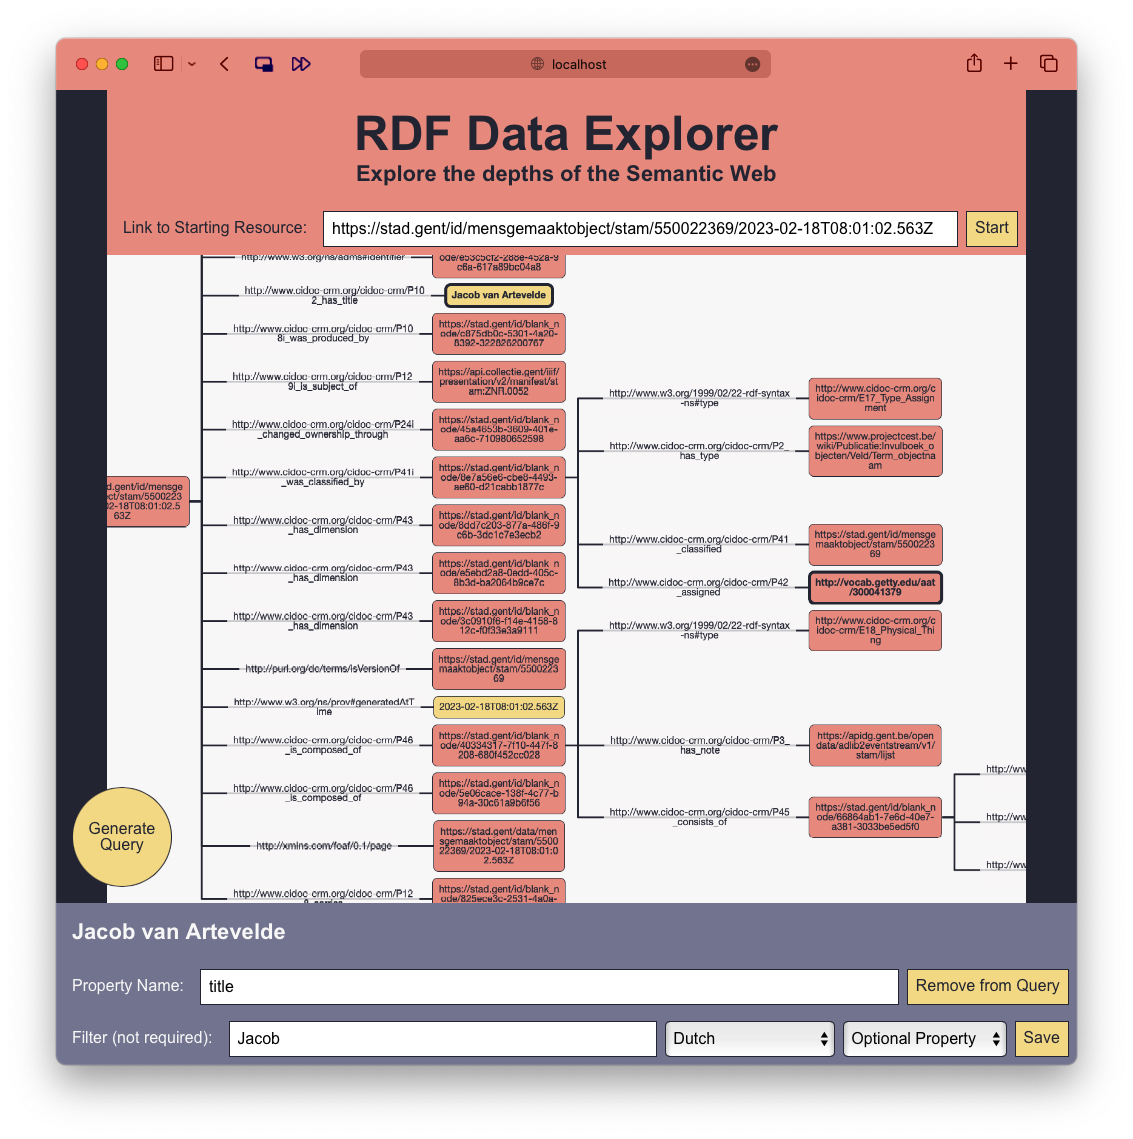
\includegraphics[width=\textwidth]{images/rdf_explorer.png}
	\caption{Screenshot of RDF Predicates Explorer}
	\label{fig:rdf_explorer}
\end{figure}

\subsection{Tree Expansion}

Another advantage to using \textit{cytoscape.js} is the ease with which event listeners for node clicks can be added. This is necessary as users need to interact with nodes. For instance, if a node represents a resource, not an atomic value, users should be able to \textit{expand} it. This involves retrieving the predicate and object for every triple pattern in which the resource is the subject. Consequently, for each such predicate-object pair found, a corresponding edge-node pair is added to the resource node. This system allows users to build a tree of predicates and resources, providing insights into the part of the web of Linked Data that the starting resource grants access to.

Naturally, behind this \textit{expanding} operation lies a SPARQL query. That query is not at all complicated, as exemplified by Code Fragment~\ref{lst:function_query_subject}. Here, the function that returns the necessary query for a given resource URI is presented. To execute the query, the application uses Comunica's standard SPARQL engine\footnote{\url{https://github.com/comunica/comunica/tree/master/engines/query-sparql}}, rather than a link traversal engine. The latter isn't necessary for this type of query, as there is no need for a link traversal engine that might needlessly search for potentially \textit{followable} links and carries some overhead anyways. Furthermore, the used query engine naturally requires a datasource. Logically, the resource URI should suffice for this. At least, that is the theory. Because in practice and as attested to in Section~\ref{sec:links_to_follow}, certain resource URIs – for various reasons – do not always lead directly to a \textit{queryable} document. For instance, Getty Vocabularies URIs only return correct JSON-LD content when a \mintinline{text}{.json-ld} extension is appended to them. Therefore, to also enable users to expand these \textit{affected} resources, the application provides the possibility to modify the datasource before executing the query from Code Fragment~\ref{lst:function_query_subject}. As a bonus, this also enables users to specify a SPARQL endpoint as the datasource, potentially speeding up querying.

\begin{listing}[htbp]
    \begin{minted}[samepage,fontsize=\small]{javascript}
function buildQuery(subjectResource) {
    return `
        SELECT ?p ?o
        WHERE {
            <${subjectResource}> ?p ?o.
        }
    `;
}
    \end{minted}
    \caption{Function returning a SPARQL query for completing a resource subject's triple pattern}
    \label{lst:function_query_subject}
\end{listing}

\subsection{Predicate Sequences Selection}

The purpose of the application central to this section is, of course, to compose queries. To achieve this, this application also utilizes the query builder application discussed in Section~\ref{sec:building_queries_predicate_sequences}. The query builder function of the latter expects several parameters, with the most important being the \mintinline{text}{properties} parameter. In other words, for each type of property the user wants to include in their query, at least the corresponding \textit{predicate sequence}, and optionally some filter details and an \mintinline{text}{optional} value, must be provided. Compiling all of this into a valid \mintinline{text}{properties} dictionary is a trivial task for the application. However, to understand the user's preferences, the necessary UI elements need to be provided. Code Fragment~\ref{fig:rdf_explorer} already provides a visual indication of those.

Specifically, the application presents an input form when a node is clicked. Initially, it only offers the option to enter a property name. The intention is for this to briefly describe the type of data obtained by following the predicate sequence to the node in question – whether a resource or an atomic value. Subsequently, once the property name is provided, the user can add the property to the query. This step presents them with a few additional yet optional fields. Specifically, the user can provide a string filter – the label of the node in question is automatically offered as an option – choose a language, and designate the property as required or optional. Each node included as a property in the query is highlighted in the tree.

Consequently, when the user is satisfied with their choices, they can press the \textit{Generate Query} button. Upon this signal, the application first collects all properties with their respective details into a dictionary, structured according to the rules defined in Section~\ref{subsec:building_queries_predicate_sequences_overview}. For each chosen node, this also requires the various predicates leading from the starting resource to that node. Fortunately, \textit{cytoscape.js} can help with this too. After all, for each node, it offers the \mintinline{text}{predecessors()}\footnote{\url{https://js.cytoscape.org/\#nodes.predecessors}} function. This leaves the application only with filtering each selected node's predecessors for just edges – predicates – and reversing their order. Eventually, once the complete \mintinline{text}{predicates} dictionary is determined, the application passes it to the query-building function, which ultimately presents the generated query to the user. As an added bonus, the application can even convert the dictionary to a JSON file, allowing it to be used as a \textit{module} in the application discussed in Section~\ref{sec:new_query_builder}.

\section{Conclusion}

The applications presented in Sections~\ref{sec:new_query_builder} and~\ref{sec:discovering_predicate_sequences} are primarily user-centric. The application in Section~\ref{sec:new_query_builder}, for instance, serves as a great starting point for absolute beginners to get a high-level idea of certain datasets, as well as how the selection of specific properties, accompanied by questions, translates into the construction of a SPARQL query. However, the drawback is that users rely on existing \textit{modules} tailored to specific datasets. Without these modules, the application has no use. This is why the application discussed in Section~\ref{sec:discovering_predicate_sequences} was developed. It allows users to select properties based on the branches and sub-branches of a specific resource in their dataset. However, this application expects a bit more technical understanding from users. Not only do users need to provide the URI of the starting resource themselves, \textit{expanding} the tree can also be a somewhat tedious process.

Certainly, both applications have their distinct strengths and weaknesses. However, the key functionality of both, which is query building, is performed by a separate application. This application provides a query-building function that enables developers to build various user-centric applications \textit{around} it. The only prerequisite is to provide the function with the appropriate parameters. Once again, the specific details of these parameters are set out in Section~\ref{subsec:building_queries_predicate_sequences_overview}.

In any case, the ultimate goal of each application discussed in this chapter is the creation of a query. The logical next step is for a user to execute this query. However, given that the generated queries are \textit{document-transcending}, users need an appropriate link traversal engine to execute them. The custom engine developed at the end of Chapter~\ref{chap:coghent_link_traversal} serves this purpose. However, it is important to note that improperly configured servers might react unexpectedly to requests from such engines, and there is thus no guarantee that every query will yield results. Temporary workarounds can however be implemented to handle such cases. For instance, the custom engine from Chapter~\ref{chap:coghent_link_traversal} can work with Getty Vocabularies resources thanks to a newly-created actor. At the time of publication, this research therefore recommends using this custom engine. 

Nevertheless, the question now becomes where users are expected to consult these engines. One option would be to manually build a standalone application \textit{around} the engine, another to simply host a \textit{Comunica SPARQL jQuery Widget}\footnote{\url{https://github.com/comunica/jQuery-Widget.js/}} with the necessary configuration. However, to save users from unnecessary copying and pasting, this research has chosen to expand the functionality of the applications from Sections~\ref{sec:new_query_builder} and~\ref{sec:discovering_predicate_sequences}. Specifically, when a query is generated in either application, users are provided with the option to execute it immediately.

This leaves only one last question to answer: what to do with these query results? Chapter~\ref{chap:handling_query_results} delves into exploring potential resolutions to the challenge of handling those.